\documentclass[12pt, a4paper]{book}

\usepackage{fancyhdr}
\usepackage[left=4cm, right=4cm, top=4cm, bottom=4cm]{geometry}
\usepackage[utf8]{inputenc}
\usepackage[table]{xcolor}
\usepackage{hyperref}
\usepackage{amsmath}
\usepackage{enumitem}
\usepackage{graphicx}
\usepackage{amsfonts}
\usepackage{color,soul}
\usepackage{booktabs}
\usepackage{subcaption}
\usepackage[justification=centering]{caption}
\usepackage{xepersian}

\DeclareMathOperator*{\argmax}{argmax}
\DeclareMathOperator*{\argmin}{argmin}
\newcolumntype{L}{>{$}l<{$}} % math-mode version of "l" column type

\newcommand{\coursetitle}{بازیابی اطلاعات}
\newcommand{\doctitle}{تمرین اول}
\newcommand{\name}{محمدرضا غفرانی}
\newcommand{\studentno}{400131076}
\newcommand{\todaydate}{\today}

\settextfont{XB Kayhan}

\pagestyle{fancy}
\lhead{\textbf{\doctitle}}
\rhead{\name}

\begin{document}

\begin{flushleft}
    \name \\
    \studentno \\
    \todaydate
\end{flushleft}

\begin{center}
    \huge
    \textbf{\coursetitle}
    \break
    \large
    \doctitle
\end{center}

% suppress the fancy header on the first page only
\thispagestyle{plain}

\section*{بخش دوم}

ابتدا توضیحات نحوه‌ پیاده‌سازی. ما تمامی حروف موجود در پیکره را به حروف کوچک تیدیل کردیم. در قدم بعدی
جملات را به توکن‌های سازنده آن تبدیل کردیم. برای علاوه بر کاراکتر فاصله از کاراکتر‌های دیگر نظیر علامت سوال و
علامت تعجب نیز استفاده کردیم. ما دو هزار کلمه پرکاربرد را برای ساختن بردار \lr{TF-IDF} استفاده کرده‌ایم.
بیشتر این کلمات به تعداد خوبی در مستندات آمده‌اند و در نتیجه می‌توانند بردار خوبی را برای مستندات
تشکیل دهند. به علاوه چون از تکنیک \lr{TF-IDF} استفاده می‌شود تاثیر کلماتی نظیر ایست‌واژه‌ها
خود به خود کم می‌شود. برای پیاده‌سازی روش \lr{TF-IDF} از کتابخانه \lr{gensim} استفاده کردیم. شیوه
ساخت مدل \lr{TF-IDF} نیز به صورت \lr{lfc} بود. سایر پارامتر‌ها همان پارامتر‌های پیش‌فرض کتابخانه است.

پس از انجام مراحل فوق، هر یک از کوئری‌های موجود در مجموعه‌داده آزمون و آموزش به بردار \lr{TF-IDF} تبدیل
می‌شود. بردار \lr{TF-IDF} تنها با استفاده از دو هزار کلمه منتخب ساخته می‌شود. در قدم بعدی شباهت کسینوسی
هر بردار موجود در داده آموزشی با داده آزمون بررسی می‌شود و شبیه‌ترین بردار‌ها به یکدیگر انتخاب می‌شوند.
در ادامه برخی از نتایج آورده شده است.

\begin{latin}
    \begin{enumerate}
        \item How will the implementation of \hl{GST} \hl{bill} \hl{impact} the lives of common people?
        \begin{itemize}
            \item Now that the \hl{GST} \hl{bill} has been passed by the Indian government, how will it \hl{impact} the lives of the common people?
            \item What are the benefits of \hl{GST} \hl{bill} for common peoples?
            \item What is the effect of \hl{GST} \hl{bill} on a common man?
        \end{itemize}
        \item I am poor in \hl{English} \hl{grammar} so how should I improve my grammar?
        \begin{itemize}
            \item How can I improve my \hl{English} \hl{grammar}?
            \item What can I do to improve my \hl{English} \hl{Grammar}?
            \item How do you learn \hl{English} \hl{grammar}?
        \end{itemize}
        \item What are some good \hl{psychological} \hl{hacks}?
        \begin{itemize}
            \item What are some \hl{psychological} \hl{hacks} for better focus?
            \item What are 20 \hl{psychological} \hl{hacks}?
            \item What are some \hl{psychological} \hl{hacks} that you can do daily?
        \end{itemize}
    \end{enumerate}
\end{latin}

\section*{بخش سوم}

\subsection*{سوال یک}

پیش‌پردازش‌های انجام شده در این قسمت مشابه پیش‌پردازش‌های قسمت قبل است.
با توجه به این که در سوال بیان شده است که از هموار‌سازی دیریکله استفاده شود؛ بنابراین نیاز است که
احتمال زیروگرام\LTRfootnote{Zerogram} نیز محاسبه شود. احتمال‌های یونیگرام\LTRfootnote{Unigram} و
زیروگرام به شرح زیر محاسبه شده است.

\begin{latin}
    \begin{eqnarray*}
        P_{\text{unigram}}(w) = \frac{\#(w)}{\sum_{x \in W} \#(x)} \hspace*{1cm} P_{\text{zerogram}}(w) = \frac{1}{|\{ x | x \in W \}|}
    \end{eqnarray*}
\end{latin}

در نوشتار بالا عملگر $\#$ تعداد کلمه مد نظر را بر می‌گرداند. منظور از $ٌW$ نیز مجموعه تمامی کلمات مشاهده شده است.

با اعمال هموارسازی دیریکله فرمول محاسبه احتمال یونیگرام به شکل زیر در می‌آید.

\begin{latin}
    \begin{eqnarray*}
        P_{unigram}(w) = \frac{\#(w) + \mu P_{\text{zerogram}}}{\sum_{x \in W} \#(x) + \mu}
    \end{eqnarray*}
\end{latin}

در فرمول بالا $\mu$ هایپرپارامتر هموارسازی است و باید تعیین شود.
در ادامه در جدول \autoref{mu_impact_p_unigram} نتایج آزمایش‌های مختلفی که برای محاسبه بهترین مقدار $\mu$
انجام شده است، آورده‌ایم. با توجه به نتایج می‌توان بیان کرد که عملکرد مدل با اندکی هموار‌سازی بهتر شده است
اما در ادامه با هموار‌سازی بیشتر عملکرد مدل بد‌تر شده است. با توجه به \autoref{mu_impact_p_unigram}
مدل در حالت $\mu=0.001$ بهترین عملکرد را داشته است، در نتیجه همین مقدار را در هنگام ارزیابی مدل در
داده‌های آزمون به کار می‌بریم.

\begin{table}
    \begin{minipage}{0.5\linewidth}
        \centering
        \caption{بررسی تاثیر $\mu$ در هموارسازی $P_{\text{unigram}}$}
        \label{mu_impact_p_unigram}
        \setLTR
        \begin{tabular}{c|c|c}
            $\mu$    & \lr{MRR} & \lr{MAP} \\
            \hline
            $0.0001$ & $0.5856$ & $0.3158$ \\
            $0.001$  & $0.5913$ & $0.3238$ \\
            $0.01$   & $0.5877$ & $0.3153$ \\
            $0.1$    & $0.5639$ & $0.2730$ \\
            $0.3$    & $0.486$  & $0.204$  \\
            $0.5$    & $0.39$   & $0.15$   \\
            $0.8$    & $0.274$  & $0.083$  \\
            $1$      & $0.2209$ & $0.0631$ \\
            $10$     & $0.0074$ & $0.0014$ \\
            $100$    & $0.0068$ & $0.0014$ \\
            $1000$   & $0.0068$ & $0.0014$ \\
        \end{tabular}
    \end{minipage}\hfill
    \begin{minipage}{0.45\linewidth}
        \centering
        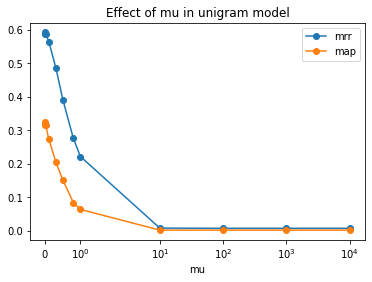
\includegraphics[width=\linewidth]{images/mu.png}
        \captionof{figure}{بررسی تاثیر $\mu$ در هموارسازی $P_{\text{unigram}}$}
    \end{minipage}
\end{table}

\begin{table}[h]

\end{table}

\subsection*{سوال دو}

پیش از ساخت مدل بایگرام، پیش‌پردازش‌های مشابهی با قسمت‌های قبلی روی داده‌ها صورت می‌گیرد.
پس از ساخت مدل بایگرام از فرمول پیشنهاد شده در صورت تمرین برای هموار‌سازی مدل استفاده شده است.
در فرمول پیشنهادی نیاز به محاسبه مدل یونیگرام نیز هست که ما مشابه قسمت قبلی آن را محاسبه کرده و
با $\mu=0.001$ هموار می‌کنیم. برای انتخاب بهترین مقدار برای پارامتر $\lambda$ از داده‌های ارزیابی استفاده می‌کنیم.
نتایج مختلف به ازای $\lambda$ در \autoref{lambda_impact_p_bigram} آورده شده است. با افزایش مقدار $\lambda$
تا $\lambda=0.3$ رفته‌رفته خروجی مدل بهبود می‌یابد اما پس از آن به دلیل همواز‌سازی بیش از حد،
عملکرد مدل افت می‌کند.

\begin{table}
    \begin{minipage}{0.5\linewidth}
        \centering
        \caption{بررسی تاثیر $\lambda$ در هموارسازی $P_{\text{bigram}}$}
        \label{lambda_impact_p_bigram}
        \setLTR
        \begin{tabular}{c|c|c}
            $\lambda$  & \lr{MRR} & \lr{MAP}    \\
            \hline
            $0.01$ & $0.585$ & $0.323$ \\
            $0.1$ & $0.582$ & $0.323$ \\
            $0.3$ & $0.603$ & $0.335$ \\
            $0.5$ & $0.596$ & $0.327$ \\
            $0.8$ & $0.595$ & $0.333$ \\
            $0.9$ & $0.591$ & $0.324$ \\
            $0.99$ & $0.584$ & $0.323$
        \end{tabular}
    \end{minipage}\hfill
    \begin{minipage}{0.45\linewidth}
        \centering
        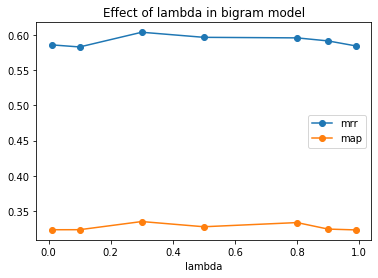
\includegraphics[width=\linewidth]{images/lambda.png}
        \captionof{figure}{بررسی تاثیر $\lambda$ در هموارسازی $P_{\text{lambda}}$}
    \end{minipage}
\end{table}

\clearpage

\section*{بخش چهارم}

در این قسمت می‌خواهیم نتایج عملکرد مدل‌ها مختلف را با هم مقایسه کنیم. نتایج به تفکیک هر
روش در \autoref{performance_evaluation} آورده شده است. از لحاظ \lr{MAP} هر سه روش عملکرد نسبتا
یکسانی داشته‌اند، بدین معنا که به طور متوسط تعداد مستندات مرتبط یکسانی را در جایگاه‌  بالا
قرار داده‌اند. در طرف مقابل از لحاظ معیار \lr{MRR} روش \lr{TF-IDF} با فاصله خوبی بهتر از دیگر
روش‌ها عمل کرده‌ است. این بدین معنی است که روش \lr{TF-IDF} به صورت متوسط مستند مرتبط را
در جایگاه بالاتری قرار داده است. مهم‌ترین عامل تاثیرگذار در این اختلاف تاثیری است که روش \lr{TF-IDF} به کلمات
مهم نسبت می‌دهد. از نگاه روش‌های یونیگرام و بایگرام کلمه کلیدی نظیر \lr{GST} تفاوتی با کلمه \lr{is} ندارد و
اتفاقا به کلمه \lr{is} به علت تعداد تکرار بیشتر احتمال بیشتری را نسبت می‌دهد. اما در روش \lr{TF-IDF}
به کلمه \lr{GST} به دلیل آن که در تعداد سند کم‌تری آمده است، امتیاز بیشتری داده می‌شود.

\begin{table}[h]
    \centering
    \caption{بررسی نتایج عملکرد روش‌های مختلف}
    \label{performance_evaluation}
    \begin{tabular}{c|c|c}
        & \lr{MRR} & \lr{MAP} \\
        \hline
        روش \lr{TF-IDF} & $0.47$ & $0.74$\\
        روش یونیگرام & $0.38$ & $0.75$ \\
        روش بایگرام & $0.38$ & $0.76$
    \end{tabular}
\end{table}

\end{document}